\section{Auswertung}
\label{sec:Auswertung}

\subsection{Bestimmung der Güteziffer}

% \subsubsection{Messdaten und Diagramm}

Die gemessenen Daten werden für die Bestimmung der in \textbf{\ref{sec:Ziel}} genannten Größen ausgewertet.
Es sei im Voraus angemerkt, dass die Messung der Leistung aufgrund von technischen Schwierigkeiten erst ab der fünften Minute erfolgen konnte. 
\\

% \begin{table}
%   \centering
%   \caption{Messdaten}
%   \label{tab:Messdaten}
%   %\sisetup{table-format=1.2}
%   %\resizebox{.5/textwidth}{!}{%
%   \begin{tabular}{c c c c c c c}  %\begin{tabular}{S[table-format=3.0] c c c c c c c[table-format=3.2]}
%     \toprule
%     {Zeit $t (\unit{\second})$} &
%     {$T_{1} (\unit{\celsius})$}&
%     {$T_{2} (\unit{\celsius})$}&
%     {$p_{a} (\unit{\bar})$}&
%     {$p_{b} (\unit{\bar})$}&
%     {$P (\unit{\watt})$} \\
%     \midrule
%        0 &    21.50 &     21.50 &       4.20 &       3.80 &      - \\
%       60 &    23.30 &     20.70 &       3.90 &       5.30 &      - \\
%      120 &    24.70 &     19.30 &       3.60 &       5.90 &      - \\
%      180 &    26.40 &     17.70 &       3.60 &       6.00 &      - \\
%      240 &    27.90 &     16.60 &       3.60 &       6.40 &      - \\
%      300 &    29.50 &     15.60 &       3.50 &       6.80 & 125.00 \\
%      360 &    31.00 &     14.60 &       3.30 &       7.00 & 125.00 \\
%      420 &    32.50 &     13.50 &       3.20 &       7.40 & 125.00 \\
%      480 &    33.80 &     12.50 &       3.00 &       7.50 & 125.00 \\
%      540 &    35.10 &     11.50 &       2.40 &       8.00 & 125.00 \\
%      600 &    36.20 &     10.60 &       2.80 &       8.10 & 125.00 \\
%      660 &    37.50 &      9.60 &       2.70 &       8.50 & 125.00 \\
%      720 &    38.50 &      8.70 &       2.80 &       8.90 & 125.00 \\
%      780 &    39.60 &      7.80 &       2.50 &       9.00 & 125.00 \\
%      840 &    40.60 &      7.10 &       2.40 &       9.10 & 115.00 \\
%      900 &    41.50 &      6.20 &       2.40 &       9.30 & 115.00 \\
%      960 &    42.40 &      5.50 &       2.20 &       9.70 & 115.00 \\
%     1020 &    43.30 &      4.70 &       2.10 &       9.90 & 115.00 \\
%     1080 &    44.10 &      4.00 &       2.10 &      10.10 & 115.00 \\
%     1140 &    44.80 &      3.30 &       2.10 &      10.20 & 115.00 \\
%     1200 &    45.60 &      2.70 &       2.00 &      10.50 & 115.00 \\
%     1260 &    46.30 &      2.10 &       2.00 &      10.80 & 115.00 \\
%     1320 &    47.10 &      1.40 &       1.90 &      11.00 & 115.00 \\
%     1380 &    47.80 &      0.80 &       1.80 &      11.10 & 115.00 \\
%     1440 &    48.40 &      0.30 &       1.80 &      11.20 & 115.00 \\
%     1500 &    49.00 &     -0.20 &       1.80 &      11.60 & 115.00 \\
%     1560 &    49.50 &     -0.70 &       1.80 &      11.80 & 115.00 \\
%     1620 &    50.00 &     -0.10 &       1.80 &      12.00 & 115.00 \\
%     \bottomrule
%   \end{tabular}
% \end{table}

% \newpage

Alle Größen wurden in SI-Einheiten umgerechnet, die Zeit für die Ausgleichsrechnung quadriert und gemäß
der Versuchsanleitung \cite{v206} den Drücken $\textit{p}_\textit{a}$ und $\textit{p}_\textit{b}$ 1 bar bzw. 100000 Pa addiert. 
\\

% \begin{table}
%   \centering
%   \caption{berechnete Werte}
%   \label{tab:berechnete_werte}
%   %\sisetup{table-format=1.2}
%   %\resizebox{.5/textwidth}{!}{%
%   \begin{tabular}{c c c c c c}  %\begin{tabular}{S[table-format=3.0] c c c c c c c[table-format=3.2]}
%     \toprule
%     {$t^{2} (\unit{\second\squared})$}&
%     {$T_{1} (\unit{\kelvin})$}&
%     {$T_{2} (\unit{\kelvin})$}&
%     {$p_{a+} (\unit{\pascal})$}&
%     {$p_{b+} (\unit{\pascal})$}& \\
%     %{$1/T_{1} (1/\unit{\kelvin})$} \\
%     \midrule
%           0.00 &  294.65 &  294.65 & 520000.00 &  480000.00 \\
%        3600.00 &  296.45 &  293.85 & 490000.00 &  630000.00 \\
%       14400.00 &  297.85 &  292.45 & 460000.00 &  690000.00 \\
%       32400.00 &  299.55 &  290.85 & 460000.00 &  700000.00 \\
%       57600.00 &  301.05 &  289.75 & 460000.00 &  740000.00 \\
%       90000.00 &  302.65 &  288.75 & 450000.00 &  780000.00 \\
%      129600.00 &  304.15 &  287.75 & 430000.00 &  800000.00 \\
%      176400.00 &  305.65 &  286.65 & 420000.00 &  840000.00 \\
%      230400.00 &  306.95 &  285.65 & 400000.00 &  850000.00 \\
%      291600.00 &  308.25 &  284.65 & 340000.00 &  900000.00 \\
%      360000.00 &  309.35 &  283.75 & 380000.00 &  910000.00 \\
%      435600.00 &  310.65 &  282.75 & 370000.00 &  950000.00 \\
%      518400.00 &  311.65 &  281.85 & 380000.00 &  990000.00 \\
%      608400.00 &  312.75 &  280.95 & 350000.00 & 1000000.00 \\
%      705600.00 &  313.75 &  280.25 & 340000.00 & 1010000.00 \\
%      810000.00 &  314.65 &  279.35 & 340000.00 & 1030000.00 \\
%      921600.00 &  315.55 &  278.65 & 320000.00 & 1070000.00 \\
%     1040400.00 &  316.45 &  277.85 & 310000.00 & 1090000.00 \\
%     1166400.00 &  317.25 &  277.15 & 310000.00 & 1110000.00 \\
%     1299600.00 &  317.95 &  276.45 & 310000.00 & 1120000.00 \\
%     1440000.00 &  318.75 &  275.85 & 300000.00 & 1150000.00 \\
%     1587600.00 &  319.45 &  275.25 & 300000.00 & 1180000.00 \\
%     1742400.00 &  320.25 &  274.55 & 290000.00 & 1200000.00 \\
%     1904400.00 &  320.95 &  273.95 & 280000.00 & 1210000.00 \\
%     2073600.00 &  321.55 &  273.45 & 280000.00 & 1220000.00 \\
%     2250000.00 &  322.15 &  272.95 & 280000.00 & 1260000.00 \\
%     2433600.00 &  322.65 &  272.45 & 280000.00 & 1280000.00 \\
%     2624400.00 &  323.15 &  273.05 & 280000.00 & 1300000.00 \\
%     \bottomrule
%   \end{tabular}
% \end{table}

% \newpage

In (\ref{fig:plot1}) werden die Temperaturverläufe in einem Diagramm dargestellt:

\begin{figure}
  \centering
  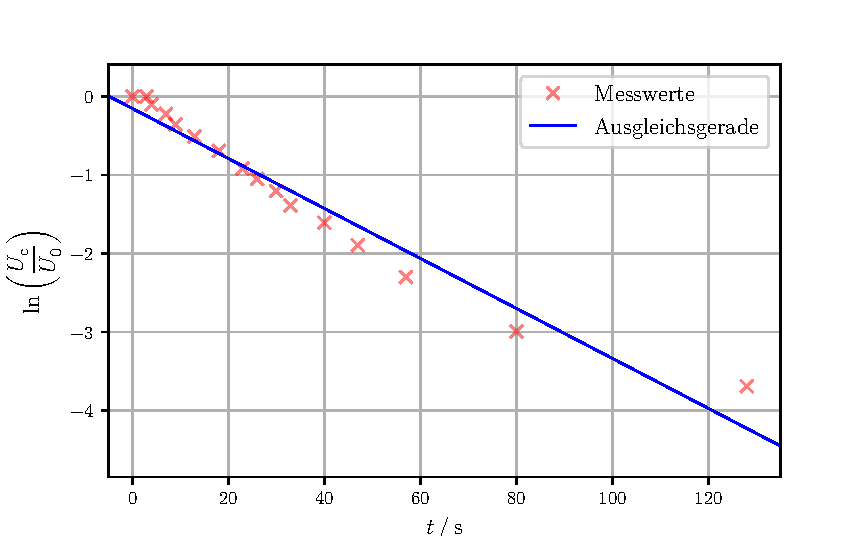
\includegraphics{plot1.pdf}
  \caption{Temperaturverläufe während der Messung}
  \label{fig:plot1}
\end{figure}

Eine nicht-lineare Ausgleichsrechnung der Temperaturverläufe mittels PYTHON mithilfe der Näherungsfunktion

\begin{equation*} 
  T(t) = At^2 + Bt + C 
\end{equation*}
\\
ergibt die folgenden Parameter für $T_{1} (\unit{\kelvin})$: \\
A = \qty{-6.6217(1407)e-6}{\unit[per-mode=reciprocal]{\kelvin\per\second\squared}} \\
B = \qty{0.0281(0002)}{\unit[per-mode=reciprocal]{\kelvin\per\second}} \\
C = \qty{294.7858(0.0825)}{\unit\kelvin} \\
\\
und für $T_{2} (\unit{\kelvin})$: \\
A = \qty{4.6346(1811)e-6}{\unit[per-mode=reciprocal]{\kelvin\per\second\squared}} \\
B = \qty{-0.0214(0003)}{\unit[per-mode=reciprocal]{\kelvin\per\second}} \\
C = \qty{294.8097(0.1062)}{\unit\kelvin} \\
% \subsubsection{Aufg. c: Bestimmung der Differentialquotienten} \label{sec:aufg_c}

Mithilfe dieser Funktionen sollen nun die Differentialquotienten $\frac{dT_{1}}{dt}$ und $\frac{dT_{2}}{dt}$ 
für vier verschiedene Temperaturen berechnet werden. Hierbei wird sich für die Temperaturen bei 
300s, 600s, 900s und 1200s entschieden. 
\\\\
Aus dem Diagramm werden die entsprechenden Steigungen über die Ableitungen der Näherungsfunktion entnommen:

\begin{align*} 
  \frac{dT}{dt} = 2At + B 
\end{align*}

Für $T_{1} (\unit{\kelvin})$ ergeben sich folgende Differentialquotienten:

\begin{table}
  \centering
  \caption{Differentialquotient für $T_{1}$}
  \label{tab:berechnete_werte_T1}
  \begin{tabular}{c c c c}
    \toprule
    {Zeit $t (\unit{\second})$} &
    {$T_{1} (\unit{\kelvin})$} &
    {$\frac{\dif{T_{1}}} {\dif{t}}$} & 
    {Gauß-Fehler $\increment \frac{\dif{T_{1}}} {\dif{t}}$}\\
    \midrule
     300.0 & 302.65 &  0.0241 &   0.0003 \\
     600.0 & 309.35 &  0.0202 &   0.0003 \\
     900.0 & 314.65 &  0.0162 &   0.0003 \\
    1200.0 & 318.75 &  0.0122 &   0.0004 \\
    \bottomrule
  \end{tabular}
\end{table}

und analog für $T_{2} (\unit{\kelvin})$:

\begin{table}
  \centering
  \caption{Differentialquotient für $T_{2}$}
  \label{tab:berechnete_werte_T2}
  \begin{tabular}{c c c c}
    \toprule
    {Zeit $t (\unit{\second})$} &
    {$T_{2} (\unit{\kelvin})$} &
    {$\frac{dT_{2}}{dt}$} &
    {Gauß-Fehler $\increment \frac{\dif{T_{2}}} {\dif{t}}$} \\
    \midrule
     300.0 & 288.75 & -0.0186 &   0.0003 \\
     600.0 & 283.75 & -0.0158 &   0.0004 \\
     900.0 & 279.35 & -0.0130 &   0.0004 \\
    1200.0 & 275.85 & -0.0103 &   0.0005 \\
    \bottomrule
  \end{tabular}
\end{table}

% \subsubsection{Aufg. d/g: Bestimmung der Güteziffer}

Aus den vier gewählten Temperaturen wird die Güteziffer $\nu$ nach (\ref{eq:Q1diff}) berechnet.
\\
Die Wärmekapazität der Kupferschlange beträgt $m_{k} c_{k}$ = 750 {\unit[per-mode=fraction]{\joule\per\kelvin}. 
Die Wärmekapazität der Wassermenge berechnet sich durch Multiplikation der Masse, hier 3 $\unit{\kilo\gram}$, mit der spezifischen
Wärmekapazität von Wasser nach \cite[278]{demtroeder1} zu $m_{w} c_{w}$ = 12546 {\unit[per-mode=fraction]{\joule\per\kelvin}. \\
\\
Für die ideale Güteziffer $\nu_{id}$ nach (\ref{eq:nu_id}) und die empirische Güteziffer nach (\ref{eq:emp_nu})
ergibt sich mit den vier Temperaturen für $T_{1}$:

\begin{table}
  \centering
  \caption{Theoretische und empirische Güteziffer der Messreihe $T_{1}$}
  \label{tab:güteziffern_t1}
  \begin{tabular}{c c c c c}
    \toprule
    {Zeit $t (\unit{\second})$} &
    Güteziffer (Theorie) &
    Güteziffer (empirisch) &
    Gauß-Fehler &
    Abweichung (\%) \\
    \midrule
     300.0 &                21.773 &                   2.563 &        0.032 &           88.23 \\
     600.0 &                12.084 &                   2.149 &        0.032 &           82.22 \\
     900.0 &                 8.914 &                   1.873 &        0.035 &           78.99 \\
    1200.0 &                 7.430 &                   1.411 &        0.046 &           81.01 \\
    \bottomrule
    \end{tabular}
\end{table}

Die Güteziffer für $T_{2}$ wird nicht erneut betrachtet, da diese im Idealfall gleich sein
müsste, hier aber geringer war. \\

\subsection{Bestimmung des Messdurchsatzes}

Der Messdurchsatz berechnet sich zunächst durch die Bestimmung der Verdampfungswärme L.
Dazu wird aus den Wertepaaren (p,T) der Messreihe und einer linearen Ausgleichsrechnung mittels PYTHON die 
Steigung und Achsenabschnitt der ermittelten Ausgleichsgerade dargestellt: 

\begin{table}
  \centering
  \caption{Steigung und Achsenabschnitt der Ausgleichsgerade}
  \label{tab:güteziffern_t1}
  \begin{tabular}{c c c}
    \toprule
    {} &         Wert &      Fehler \\
    \midrule
    Steigung m        & -2651.537 &  97.560 \\
    Achsenabschnitt b &     9.203 &   0.313 \\
    \bottomrule
  \end{tabular}
\end{table} 

Die Verdampfungswärme ergibt sich aus L = $-m \cdot R$, wobei m die Steigung der Geraden und R die 
allgemeine Gaskonstante ist. Das negative Vorzeichen rührt von der negativen Steigung. 
\\

Somit ergibt sich für die Verdampfungswärme:
$L$ = \qty{22046.074(811.158)}{\unit[per-mode=fraction]{\joule\second\per\mol\kelvin}}.

\begin{figure}
  \centering
  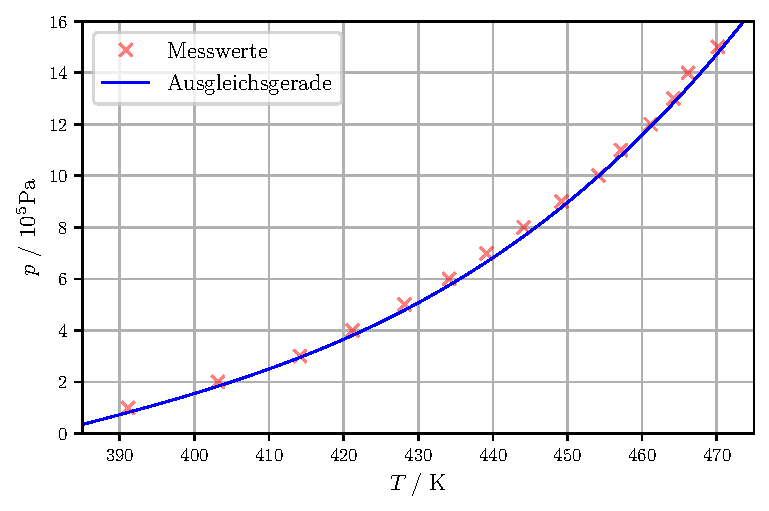
\includegraphics{plot2.pdf}
  \caption{Logarithmischer Druckverlauf des Drucks $p_{b}$}
  \label{fig:plot2}
\end{figure}

In Tabelle \ref{tb:massendurchsaetze} sind die nach (\ref{eq:massendurchsatz}) berechneten Massendurchsätze:

\begin{table} 
  \centering
  \caption{berechneter Massendurchsatz}
  \label{tb:massendurchsaetze}
  \begin{tabular}{c c c c c c}
    \toprule
    {Zeit $t (\unit{\second})$} &
    {$\frac {\dif{Q_{2}}} {\dif{t}}$} &
    {$\frac {\dif{m}} {\dif{t}} (\unit[per-mode=fraction]{\mol\per\second})$} &
    {Gauß-Fehler $\increment \frac {\dif{m}} {\dif{t}} (\unit[per-mode=fraction]{\mol\per\second})$} &
    {$\frac{\dif{m}} {\dif{t}} (\unit[per-mode=fraction]{\gram\per\second})$} &
    {Gauß-Fehler $\increment \frac {\dif{m}} {\dif{t}} (\unit[per-mode=fraction]{\gram\per\second})$} \\
    \midrule
     300.0 & -247.3056 &        -0.0112 &          0.0008 &      -1.3542 &        0.0967 \\
     600.0 & -210.0768 &        -0.0095 &          0.0007 &      -1.1486 &        0.0846 \\
     900.0 & -172.8480 &        -0.0078 &          0.0006 &      -0.9431 &        0.0725 \\
    1200.0 & -136.9488 &        -0.0062 &          0.0005 &      -0.7496 &        0.0605 \\
    \bottomrule
\end{tabular}
\end{table}

Für weitere Berechnungen soll der Massendurchsatz nun noch in SI-Einheiten umgewandelt. Dafür wird mit der molaren Masse
120,91 $\unit[per-mode=fraction]{\gram\per\mol}$ von Dichlordifluormethan multipliziert. 


\subsection{Bestimmung der mech Kompressorleistung $N_{mech}$}

Die Gasdichte $\rho$ lässt sich aus dem in der Versuchsanleitung \cite[7]{v206} angegebenen Wert 
$p_{0}$ = 5,51 g/l (Dichlordifluormethan) und der idealen Gasgleichung berechnen:

\begin{align*}
  pV = nRT \iff \frac{pV}{T} = nR
\end{align*}

mit R = 8,3144508 \unit[per-mode=fraction]{\joule\second\per\mol\kelvin}, $p_{0}$ = 1 bar, $\kappa$ = 1,14 und
$T_{0}$ = 0\unit{\celsius} = 273,14\unit{\kelvin}\\
\\
aus $nR$ = const., also $n_{1}R$ = $n_{2}R$, folgt:

\begin{align*}
  \frac{p_{0}V_{0}}{T_{0}} = \frac{p_{2}V_{2}}{T_{2}}
\end{align*}

Mit $\rho V \iff V = \frac{m}{\rho}$ folgt:

\begin{align*}
  \frac{p_{0}\cancel{m}}{\rho_{0}T_{0}} = \frac{p_{2}\cancel{m}}{\rho_{2}T_{2}}
\end{align*} \\

Somit folgt mit $\rho_{0} = \rho$ und $p_{2} = p_{a}$ schließlich:

\begin{align}
  \frac{p_{0}}{\rho_{0}T_{0}} = \frac{p_{a}}{T_{2}\rho} \iff \rho = \frac{p_{0}T_{0}p_{a}}{T_{2}p_{0}}
\end{align}\\

Damit folgt aus Gleichung (\ref{eq:n_mech}):

\begin{equation*}
  N_\text{mech} = 
  \frac{1}{\kappa - 1} 
  \left(\text{p}_\text{b} \sqrt[\kappa]{\frac {\text{p}_\text{a}} {\text{p}_\text{b}}} - \text{p}_\text{a} \right)
  \frac{1} {\frac {\rho_{0}T_{0}p_{a}} {T_{2}p_{0}}} \frac{\increment m}{\increment t} 
  =
  \frac{1}{\kappa - 1} 
  \left(\text{p}_\text{b} \sqrt[\kappa]{\frac {\text{p}_\text{a}} {\text{p}_\text{b}}} - \text{p}_\text{a} \right)
  \frac {T_{2}p_{0}} {\rho_{0}T_{0}p_{a}} \frac{\increment m}{\increment t}
\end{equation*} \\

Die mechanische Leistung des Kompressors beträgt somit:

\begin{table}
  \centering
  \caption{Gasdichte \rho und mechanische Leistung $N_\text{mech}$ (\unit{\watt})}
  \label{tab:massendurchsaetze}
  \begin{tabular}{c c c c}
    \toprule
    {Zeit $t (\unit{\second})$} &
    {Dichte $\rho$ $(\unit[per-mode=fraction]{\gram\per\cubic\meter})$} &
    {Leistung $N_\text{mech} (\unit{\watt})$} &
    {Gauß-Fehler $\increment N_\text{mech} (\unit{\watt})$} \\
    \midrule
     300.0 &               23.455 &        -12.969 &    0.926 \\
     600.0 &               20.156 &        -17.510 &    1.290 \\
     900.0 &               18.318 &        -18.232 &    1.402 \\
    1200.0 &               16.368 &        -17.607 &    1.421 \\
    \bottomrule
    \end{tabular}
\end{table}

Es fällt auf, dass die mechanische Leistung negativ ist. Dies rührt von dem negativen Massendurchsatz wie der
Tabelle (\ref{tb:massendurchsaetze}) entnommen werden kann. 
Aus dem Zusammenhang soll dieses Ergebnis als die tatsächlich positive Leistung interpretiert werden, die dem System zugefügt wird.